\subsection{Umelá inteligencia}\label{subsec:ai}

Od počiatku vzniku mechanických strojov, ktoré pomáhajú ľuďom pri svojej práci sa pri nich nepriamo niesol aj pojem
\enquote{umelá inteligencia}.
Medzi odbornou verejnosťou tento pojem stále nie je jednotný, no väčšina z nich má rovnakú myšlienku:
inteligencia vykonávaná strojmi (narozdiel od prirodzenej inteligencie, ktorú vykonávajú ľudia, či
zvieratá).\cite{ai_definition}
Ak stroj (aj mechanický) dokáže niečo vykonať bez explicitne zadaného príkazu, je považovaný za inteligentný.

\subsubsection{Metódy}

Umelá inteligencia (angl. artificial intelligence) je široká vedná disciplína, ktorá zahŕňa\cite{ai_methods}
\begin{itemize}
    \item \textbf{fuzzy prístup} k riešeniu nejasných úloh (napr. optimalizácia pri skladových zásobách, ktoré sú nejasné)
    \item \textbf{pravdepodobnostné grafické modely}: markovove modely, skryté markovove siete, apod.
    \item \textbf{rozhodovacie stromy} medzi ktoré patrí klasifikácia a regresia
    \item \textbf{učenie na báze komisií}: výsledok sa určuje na základe "hlasovania" viacerých modelov
    \item \textbf{učenie s odmenou}: odmeňovanie dobrých výsledkov
    \item \textbf{expertné systémy}
    \item \textbf{logické systémy}: odvodzovanie v logike
    \item \textbf{matematická optimalizácia} (spojitá, diskrétna, \dots)
    \item \textbf{prehľadávanie stavového priestoru} (napr. minimax)
    \item \textbf{analýza jazyka}: textová analýza, oprava pravopisu, predikcia, preklad, generovanie konspektu, atď.
    \item \textbf{dátová analýza}
    \item a mnoho ďalšieho
\end{itemize}
Metódy niektorých skupín sa môžu prelínať (napr. na analýzu obrazu a na analýzu zvuku je možné použiť umelé neurónové
siete).\cite{ai_ann_sound,ai_ann_image}
Dôsledkom toho je aj fakt, že niektoré metódy sa používajú viac a iné menej.
Využiteľnosť a efektivita metód závisí teda najmä od problému, ktorý riešia.

Ak je problémom plánovanie trasy pre kuriérov, použije sa matematická optimalizácia.
Ukážkou použitia môže byť ako americká spoločnosť UPS v amerických mestách, kde je systém ulíc riešený kolmým spôsobom,
čo najviac obmedzila zatáčanie kuriérov \emph{vľavo}.\cite{ups_optimization}
Dôvodom je najmä to, že keď kuriér odbočuje vľavo, musí dať prednosť protiidúcim vozidlám, pričom auto stojí na
križovatke naštartované, nečinné a plytvá pohonnými hmotami.
Dôsledkom sú nasledovné vylepšenia:
\begin{enumerate}
    \item ušetrených takmer 40 miliónov litrov paliva ročne
    \item o 100 tisíc ton $CO_2$ menej
\end{enumerate}
Rovnaké vylepšenia by prinieslo odstavenie 21 tisíc áut.

Na druhú stranu, keď sa rieši problém rozpoznávania hlasových príkazov, je nutné problém rozdeliť na 2 podproblémy:
\begin{enumerate}
    \item \emph{spracovanie zvuku}, napr. s využitím skrytých Markovových modelov\cite{hmm}
    \item \emph{spracovanie textu}\cite{text_analysis}
\end{enumerate}

Je teda zjavné, že algoritmus, ktorý rozpoznáva význam textu nebude stačiť pre plánovanie trás kuriérov a naopak.

Nižšie sú popísané metódy, ktoré sú v rámcu umelej inteligencie využívané najlepšie.

\paragraph{Heuristické metódy}

Heuristiky sú často používanou metódou vo vyhľadávacích algoritmoch.\cite{heuristic}
Na rozdiel od exaktných algoritmov, ktoré prehľadávajú celý priestor riešení, heuristiky prehľadávajú len okolie
východiskového riešenia.
Ak napríklad je cieľom heuristiky nájsť minimum nejakej funkcie (nemusí byť zadaná analyticky) v $n$-rozmernom priestore,
dokáže táto metóda nájsť len lokálne minimum v závislosti od toho, v akom bode sa nachádza východzie riešenie.
Príklad je uvedený pre funkciu
\begin{equation}
    f(x,y)=e^{\cos(x)+\sin(y)}\frac{x+y}{30}+\frac{5}{2}
\end{equation}
kde $x\in<-12,12>$, $y\in<-12,12>$.
\begin{figure}[H]
    \centering
    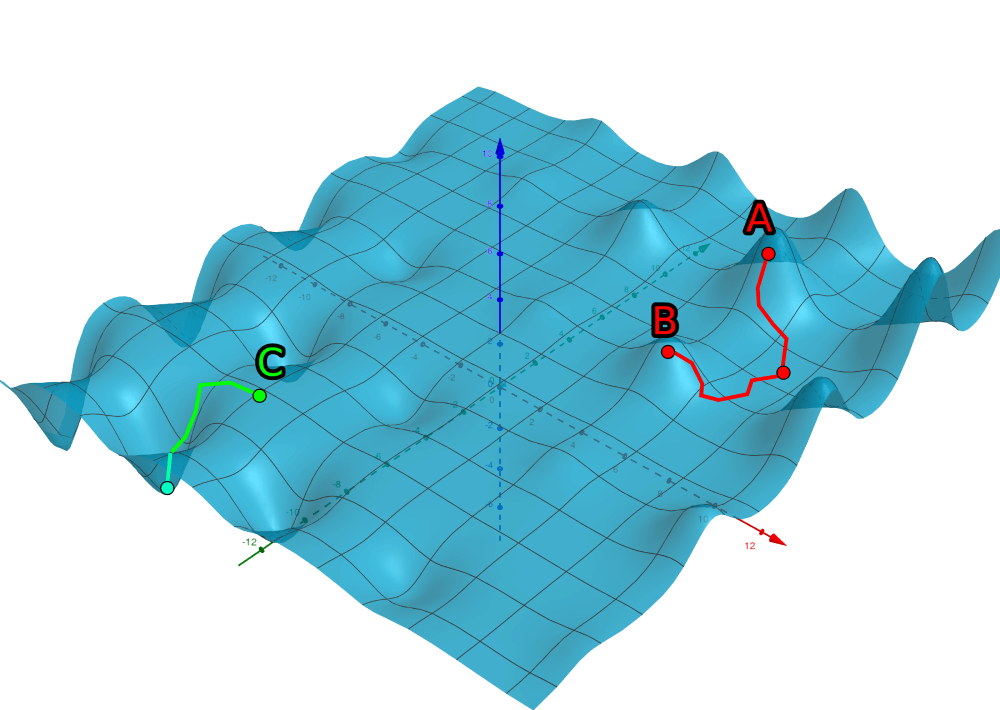
\includegraphics[width=0.8\textwidth]{images/heuristic.png}
    \caption{Heuristika a jej riešenia v závislosti od východzieho riešenia}
\end{figure}\label{figure:heuristic-method}
Pri nastavení východiskového bodu \textbf{A} alebo \textbf{B} nájde heuristika rovnaké lokálne minimum (čo sa môže javiť
ako globálne), no pre východzí bod \textbf{C} nájde algoritmus globálne minimum, čo ale nie je možné overiť bez
prehľadania celého priestoru riešení.
Z toho je možné usúdiť, že riešenie heuristiky nie je vždy optimálne a nikdy jeho optimálnosť nie je zaručená.
Na druhú stranu sú heuristiky extrémne rýchle oproti exaktným algoritmom.
Heuristické metódy patria medzi najzákladnejšie techniky v rámci umelej inteligencie.

Ako ukážkový príklad praktického využitia heuristických metód je možné uviesť hľadanie najkratšej (alebo najrýchlejšej)
cesty medzi dvoma mestami v cestnej sieti Slovenska pre navigačné systémy alebo pohyb neovládaných postáv v hrách
(angl. non-player character, skr. NPC - akákoľvek postava v hre, ktorú neovláda človek).
Pre oba tieto príklady je možné použiť napríklad \emph{A* algoritmus}.\cite{heuristic}

\paragraph{Metóda podporných vektorov}

Anglicky support vector machine (skr. SVM) je metóda strojového učenia s učiteľom (reinforcement
learning).\cite{support_vector_machine}
Cieľom tejto metódy je nájsť takú \emph{nadrovinu} v $n$-rozmernom vyhľadávacom priestore, ktorá vstupné dáta rozdelí
do dvoch podpriestorov.
Metóda je určená pre klasifikáciu a regresnú analýzu.
Ak je metóda konštruovaná ako optimalizačná úloha jej účelová funkcia vyzerá podobne ako nasledovná:
\begin{equation}
    \max \sum_{\forall i}{\sqrt{\sum_{\forall j}{(\vec{v}_j - x_{ij})^2}}}
\end{equation}
Kde $\vec{v}$ je hľadaný vektor a $\vec{v}_j$ sú jeho zložky a kde $x_i$ je vzorka zo vstupných dát a $x_{ij}$ sú jeho
zložky.
Keďže výraz $\sqrt{\sum_{\forall j}{(\vec{v}_j - x_{ij})^2}}$ vyjadruje najmenšiu vzdialenosť medzi vektorom a
vzorkou, dá sa povedať, že metóda hľadá takú nadrovinu, ktorá priestor riešení rozdelí čo najlepšie, resp. tak, aby
najmenšia vzdialenosť bodu od nadroviny bola čo najväčšia (maximálna)
\begin{figure}[H]
    \centering
    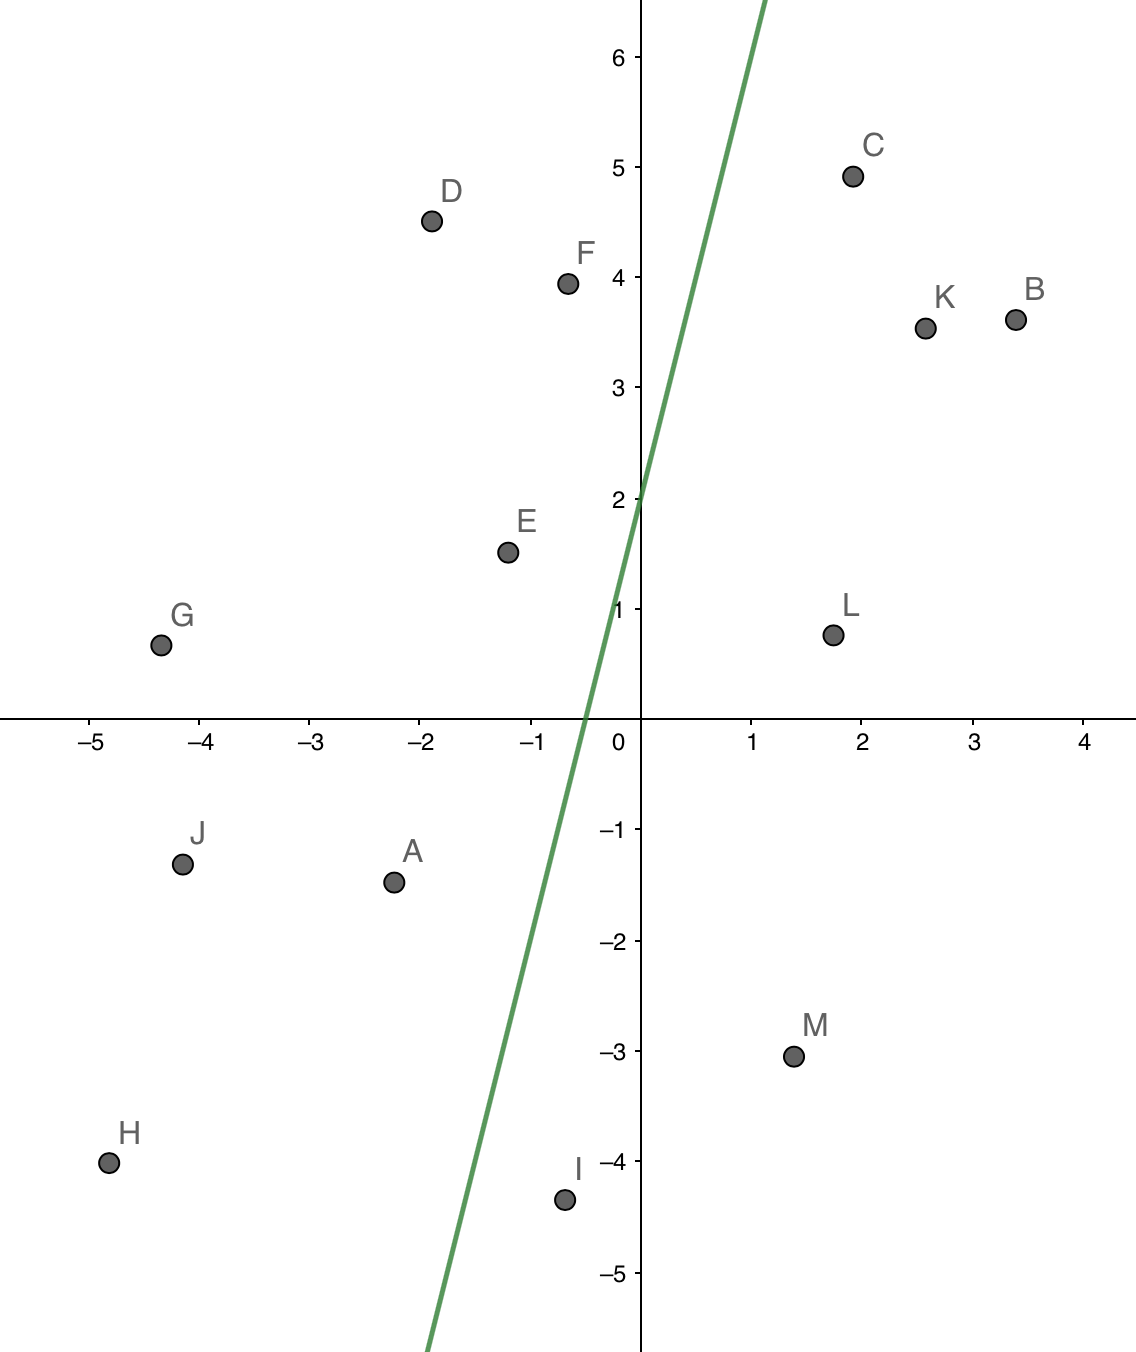
\includegraphics[width=0.5\textwidth]{images/svm.png}
    \caption{Support vector machine}
\end{figure}\label{figure:svm}

Typickým príkladom použitia metódy podporných vektorov je rozdelenie e-mailovej komunikácie do dvoch skupín: relevantnú
a nevyžiadanú poštu (spam), no podporné vektory sa dajú použiť aj na spracovanie obrazu, či textu.

\paragraph{Umelé neurónové siete}

Umelé neurónové siete (skr. ANN, z angl. artificial neural networks) je metóda umelej inteligencie vychádzajúca z
biologických (prirodzených) neurónových sietí.
Pre túto metódu je špecifická najmä jej štruktúra, ktorá sa dá reprezentovať grafom a teda je jednoduchá na pochopenie.
Umelé neurónové siete sú jednou z najrozšírenejších metód a majú výborne spracované matematické pozadie, vďaka ktorému
sú v riešení svojho problému efektívne v súvislosti s výkonom a výpočtovým časom no aj so správnosťou riešenia.
Na druhú stranu výstupy z umelých neurónových sietí sú porovnateľné s heuristickými a metaheuristickými metódami, tzn.
nie vždy je umelá neurónová sieť vo svojom výsledku správna.
Riešenie na jej výstupe je teda suboptimálne.
Zároveň je pri tejto metóde nutné dbať na jej štruktúru, ktorá je vždy špecifická pre daný problém a je nutné túto
štruktúru navrhnúť a vyladiť tak, aby dobre riešila daný problém.
Umelé neurónové siete sú bližšie popísané v \autoref{subsec:algo-ann}.

\paragraph{MiniMax}

Tento algoritmus patrí medzi metódy prehľadávanie stavového priestoru.
Základným princípom tejto metódy je \textbf{mini}malizácia úžitku oponenta v hre a \textbf{max}imalizácia úžitku
cieľového hráča.
Ak z každého stavu (najmä) hry sa dá do ďalšieho stavu dostať zmenou jednej premennej (z $n$ premenných),
vytvorí sa na základe pravidiel stavový strom (resp. rozhodovací strom), cieľový stav (list) sa ohodnotí reálnym číslom
a na základe toho sú ohodnotené aj stavy až kým algoritmus nepríde do koreňa.
Z koreňa je potom jasné, do ktorého stavu sa presunúť, aby úžitok cieľového hráča bol čo najväčší (maximálny).
Metóda Minimax je bližšie popísaná v \autoref{subsec:algo-minmax}.
\\
\\
V súčasnom stave je teda jednoduché vytvoriť, analyzovať a implementovať už vytvorené algoritmy a transformovať ich
do ktoréhokoľvek prostredia (napr. aj Cave).
Na základe zamerania aplikácie boli pre implementáciu zvolené \emph{umelé neurónové siete}, ktoré sú bližšie popísané v
\autoref{subsec:algo-ann} a ako rozhodovacie pravidlo v teórii hier pri vyhľadávacích stromoch často využívaný
algoritmus \emph{minimax} (viac v \autoref{subsec:algo-minmax}).
